\section{Resultados en Xschem, con los parámetros obtenidos del amplificador tipo \textit{folded cascode} \label{sec:s4}}

\begin{center}
	\begin{minipage}{12cm}
		\begin{tcolorbox}[title=Actividad 2]
			Utilizando el simulador NGSPICE en la herramienta de Xschem, simular el amplificador operacional \textit{folded cascode} con las razones $\frac{W}{L}$ calculadas previamente.
		\end{tcolorbox}	
	\end{minipage}
\end{center}

\begin{equation*}
	\begin{array}{l l}
		\textbf{Resultados obtenidos de la simulación} \\
		A_{V} = \frac{A_{V}(0)}{R \times C} = \frac{ 8.495026 }{ 100000.0 \times 1.2e-08 } \\
		A_{V} =  5663.350973  \\
		P_{diss} = V_{DD} \times (I_{9}+I_{10}) =  1.8 \times ( 0.000165  +  0.000165 ) \\
		P_{diss} =  0.594  mW \\
		GB =  105.841211  KHz \\
		Slew Rate =  5.214511 \frac{V}{\mu s} \\
	\end{array}
\end{equation*}

\begin{figure}[ht]
	\centering
	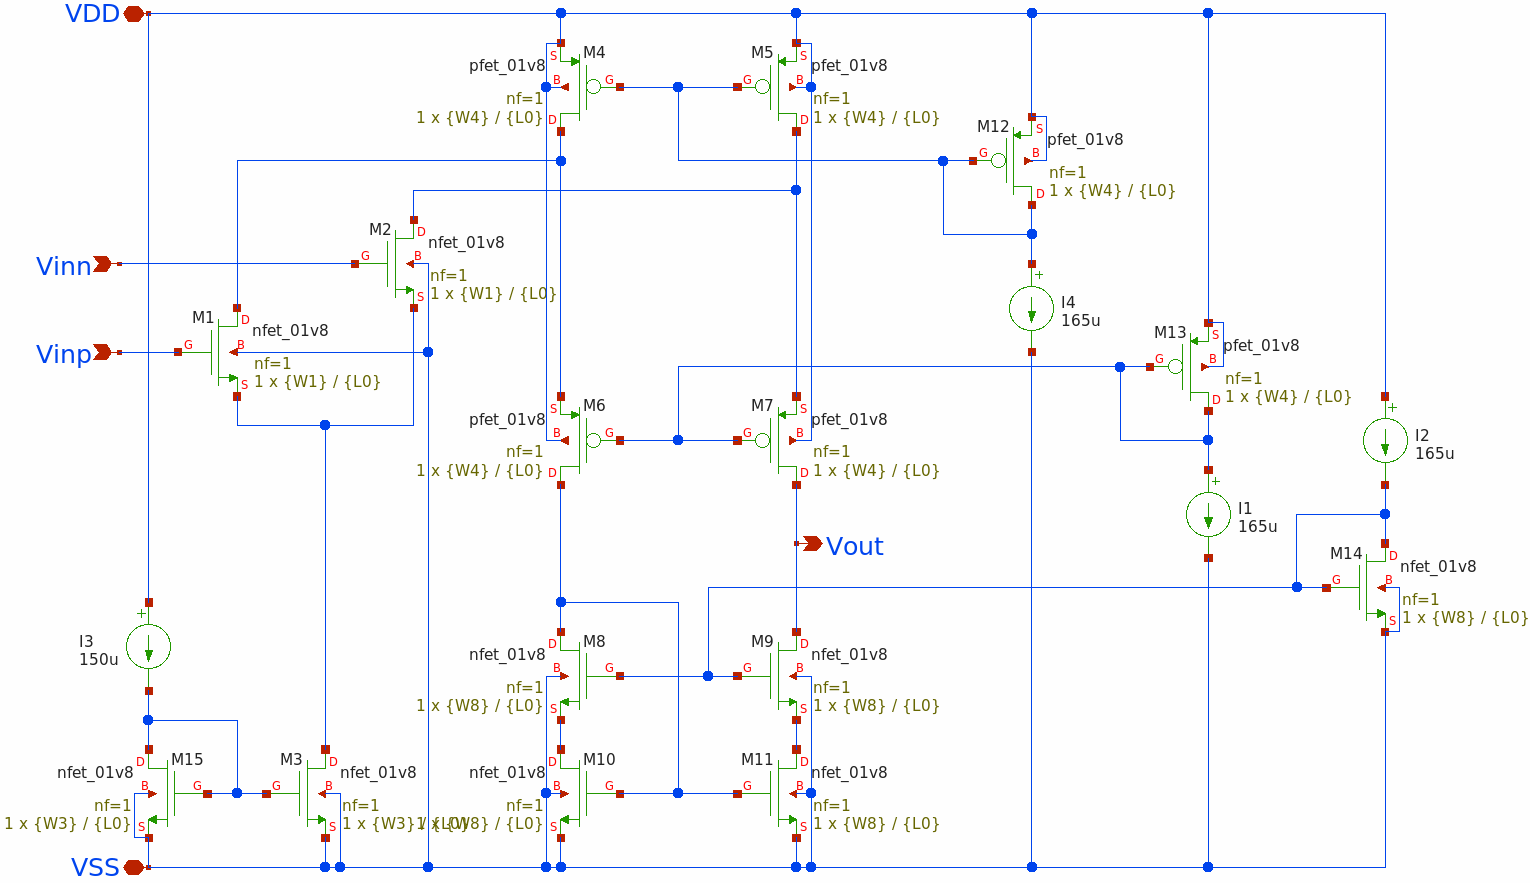
\includegraphics[scale=0.3]{FoldedOneStageOpAmp.png}
	\caption{Diagrama esquemático del amplificador operacional \textit{folded cascode} de una etapa. \label{fig:FoldedOneStageOpAmp}}
\end{figure}

\begin{figure}[ht]
	\centering
	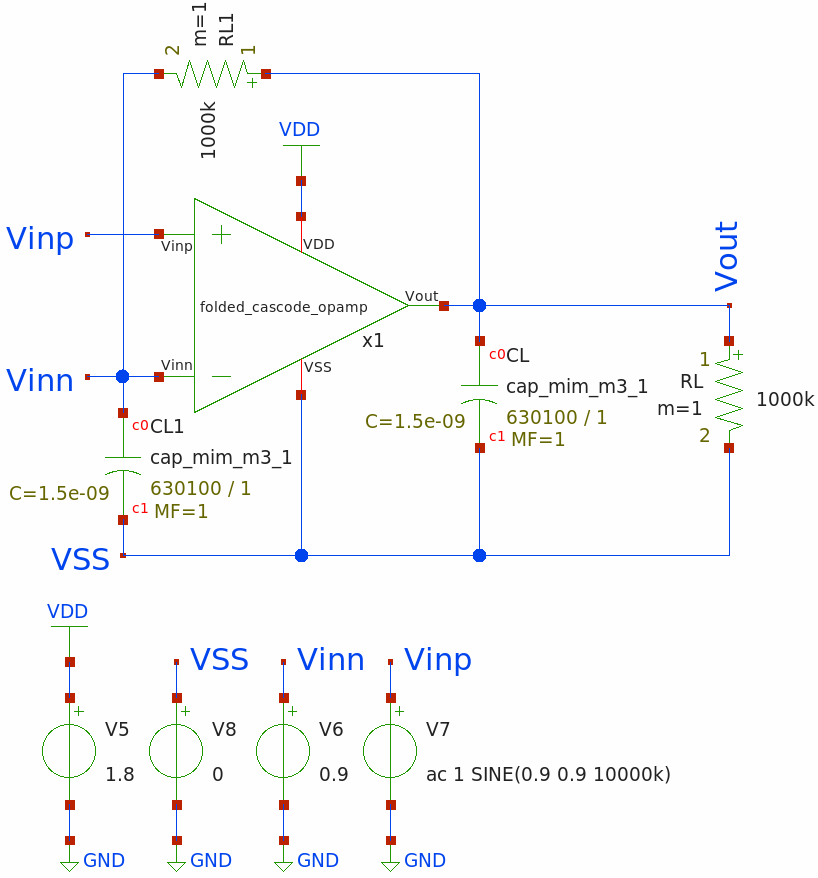
\includegraphics[scale=0.34]{FoldedOneStageOpAmpAv.png}
	\caption{Circuito utilizado para obtener la ganancia del amplificador operacional \textit{folded cascode} de una etapa. \label{fig:FoldedOneStageOpAmpAv}}
\end{figure}

\begin{figure}[ht]
	\centering
	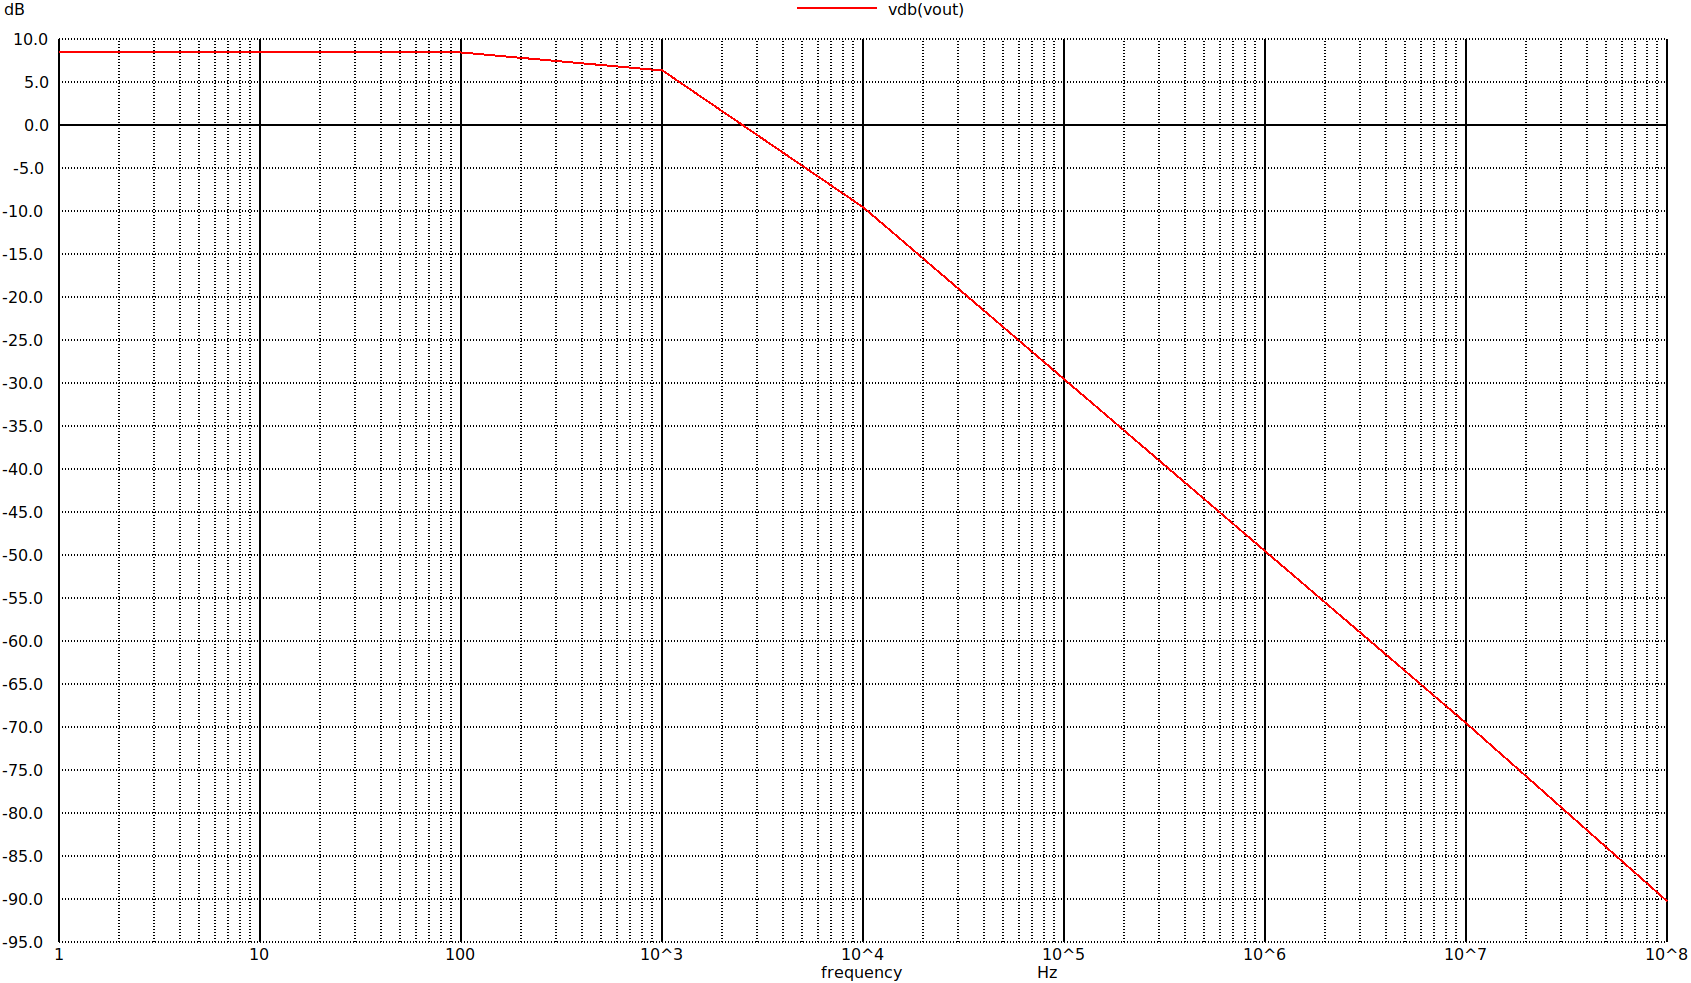
\includegraphics[scale=0.28]{FoldedOneStageOpAmpAvWave.png}
	\caption{Diagrama de Bode obtenido de la \autoref{fig:FoldedOneStageOpAmpAv}. \label{fig:FoldedOneStageOpAmpAvWF}}
\end{figure}

\begin{figure}[ht]
	\centering
	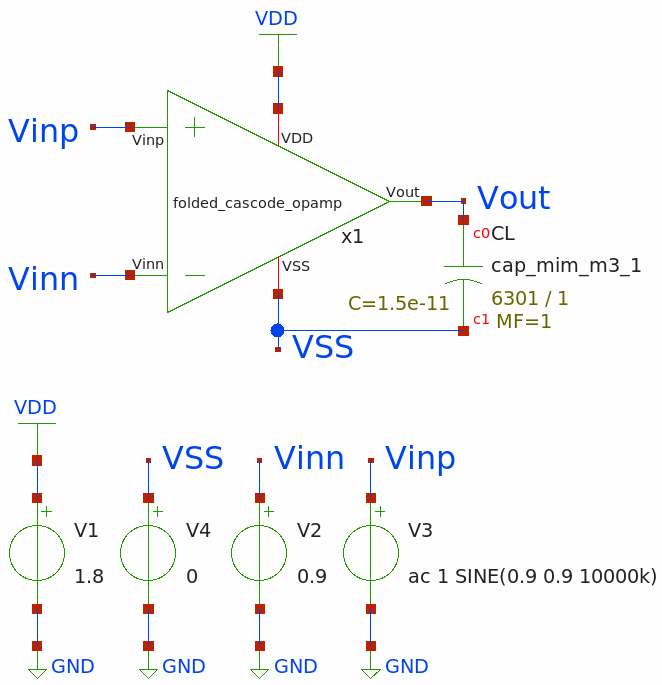
\includegraphics[scale=0.43]{FoldedOneStageOpAmpGB.png}
	\caption{Circuito utilizado para obtener la ganancia en ancho de banda (\textit{Gain Bandwidth}) del amplificador operacional \textit{folded cascode} de una etapa. \label{fig:FoldedOneStageOpAmpGB}}
\end{figure}

\begin{figure}[ht]
	\centering
	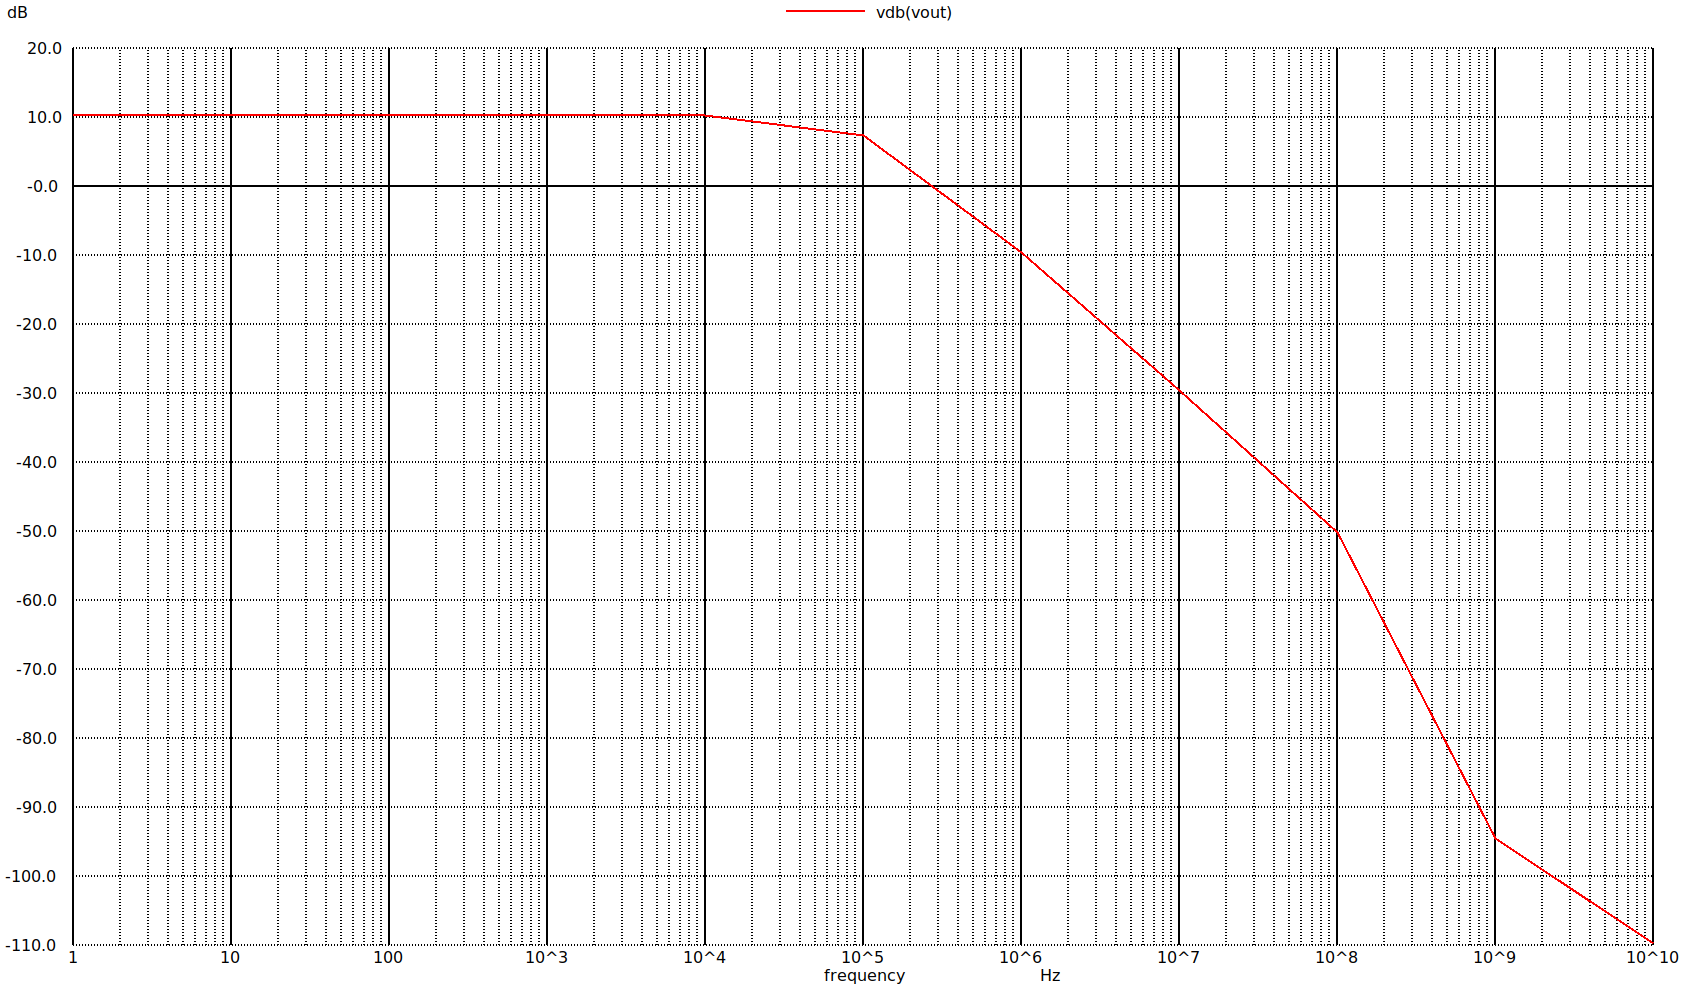
\includegraphics[scale=0.28]{FoldedOneStageOpAmpGBWave.png}
	\caption{Diagrama de Bode obtenido de la \autoref{fig:FoldedOneStageOpAmpGB}. \label{fig:FoldedOneStageOpAmpGBWF}}
\end{figure}

\begin{figure}[ht]
	\centering
	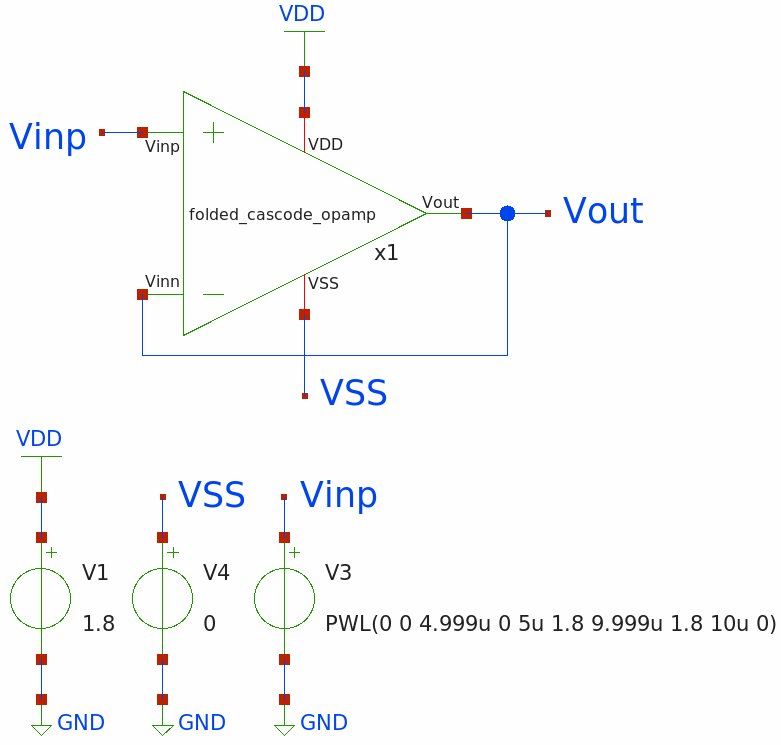
\includegraphics[scale=0.4]{FoldedOneStageOpAmpSR.png}
	\caption{Circuito utilizado para evaluar obtener el \textit{Slew Rate} del amplificador operacional \textit{folded cascode} de una etapa (seguidor de voltaje). \label{fig:FoldedOneStageOpAmpSR}}
\end{figure}

\begin{figure}[ht]
	\centering
	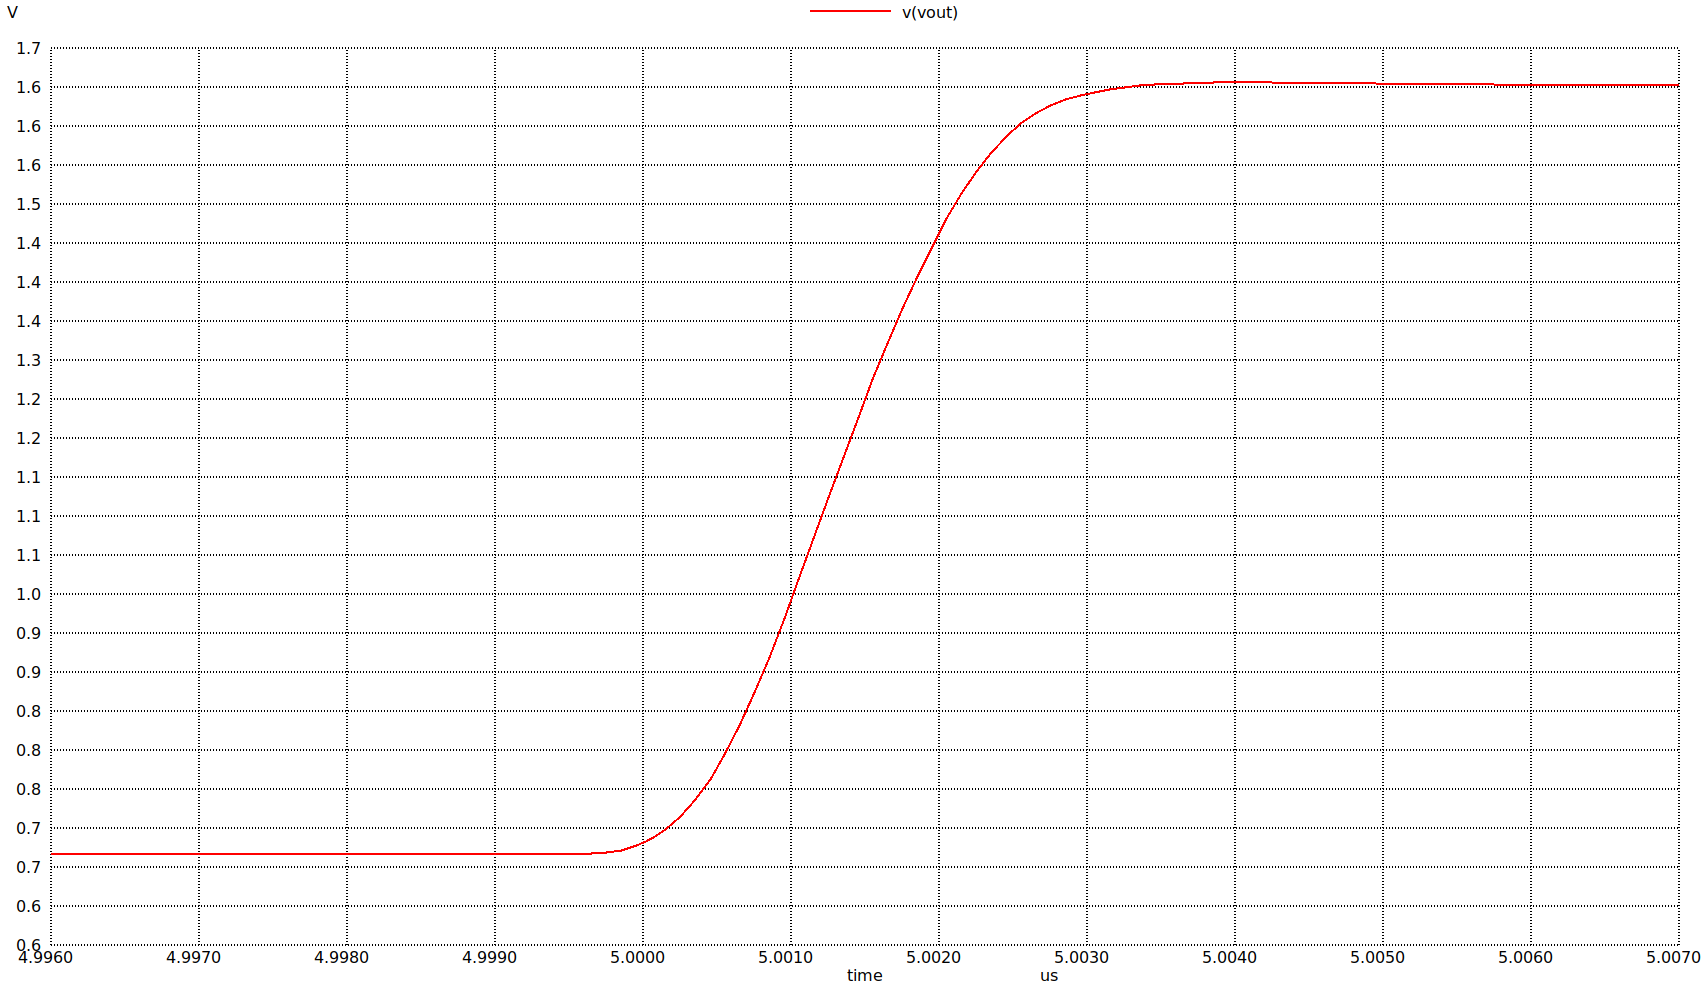
\includegraphics[scale=0.28]{FoldedOneStageOpAmpSRWave.png}
	\caption{Gráfica del voltaje de salida obtenido de la \autoref{fig:FoldedOneStageOpAmpSR}. \label{fig:FoldedOneStageOpAmpSRWF}}
\end{figure}